% nie rusza�
\RequirePackage{ifpdf}
\newif\ifelektroniczna
\newif\ifjednostronna
\newif\ifprojektInzynierski

%%%%%%%%%%%%%%%%%%%%%%%%%%%%%%%%%%%%%%%%%%%%%%%%%%%%%%%%%%%%%%%%%%%%%%%%%%%%
% USTAWIENIA GLOBALNE I domy�lna �cie�ka do plik�w z obrazkami, kodowanie itp. 
% okre�lone s� w drugiej sekcji ustawie�

% czy projekt czy praca magisterska
\projektInzynierskitrue % projekt
%\projektInzynierskifalse % praca magisterska

% czy wersja elektroniczna (pdf z kolorowymi linkami) czy nie (np. do druku)
\elektronicznatrue
%\elektronicznafalse

% czy jednostronna (recenzent), czy dwustronna (do akt);
% UWAGA: to nie jest dyrektywa dla drukarki; nie zmienia sposobu wydruku, 
% tylko to, w jaki spos�b rozpoczynane s� rozdzia�y, ustawiane marginesy
% itp.

\jednostronnafalse
%\jednostronnatrue

%%%%%%%%%%%%%%%%%%%%%%%%%%%%%%%%%%%%%%%%%%%%%%%%%%%%%%%%%%%%%%%%%%%%%%%%%%%%


% nie rusza�
\ifjednostronna
    \def\strony{oneside,openany}
\else
    \def\strony{twoside,openright}
\fi

\ifpdf
    % uwaga, ustawiaj�c co� innego ni� 12 sprawd� uk�ad strony tytu�owej (marginesy)
    \documentclass[pdftex,12pt,a4paper,\strony,colorlinks,nocenter,noupper,crosshair]{thesis}
    \usepackage[pdftex]{graphicx}
    \pdfcompresslevel=1
\else    
    \documentclass[12pt,a4paper,\strony,nocenter,noupper,crosshair]{thesis}
    \usepackage{graphicx}
\fi

% nie rusza�
\usepackage{url}
\usepackage{stronatytulowa}

%%%%%%%%%%%%%%%%%%%%%%%%%%%%%%%%%%%%%%%%%%%%%%%%%%%%%%%%%%%%%%%%%%%%%%%%%%%%
% USTAWIENIA GLOBALNE - cz�� 2
%

% kodowanie dokumentu
%\usepackage[utf8]{inputenc}   % linuks/windows/mac; pozwala na �atwe mieszanie znak�w z r�nych j�zyk�w
\usepackage[cp1250]{inputenc} % windows

% dane 
\ifprojektInzynierski
    \def\rodzaj{Projekt in�ynierski}
\else
    \def\rodzaj{Praca dyplomowa magisterska}
\fi
%\def\rodzaj{Praca przej�ciowa}

% stan na 2011-2012
\ifprojektInzynierski
    \def\wydzial{Automatyki Elektroniki i~Informatyki}
\else
    \def\wydzial{In�ynierii Biomedycznej}
\fi

\def\tytul{TYTUL \\PRACY} % Prosz� u�y� i ma�ych, i du�ych liter!
\def\autor{Autor: AUTOR PRACY} %Jan Kowalski a NIE JAN KOWALSKI

% tytu� i autor dla pdfa - najcz�ciej jw, ale bez podzia�u na liniie i BEZ POLSKICH LITER
\def\tytulpdf{TYTUL DLA PDFa}
\def\autorpdf{AUTOR DLA PDFa}

% promotor
\def\promotor{Kieruj�cy prac�: PROMOTOR} % prof. nzw. dr hab. in�. dr n.med doc. Jan Kowalski

% z konsultantem/bez konsultanta
%\def\konsultant{Konsultant: Konsultant} prof. nzw. dr hab. in�. dr n.med doc. Jan Nowak
\def\konsultant{}

\def\data{Gliwice, MIESI�C, ROK} % uwaga na wielko�� liter: grudzie� 2012/czerwiec 2012/..

% do pdfa
\def\slowakluczowe{SLOWA,KLUCZOWE}

% �cie�ka do obrazk�w
\graphicspath{{./rysunki/}}

% ustawienia dla pdfa
\ifpdf
\ifelektroniczna
     \usepackage[pdfusetitle=true,
	  pdfsubject={\tytulpdf},
	        pdfkeywords={\slowakluczowe}, 
		pdfcreator={\autorpdf},
		pdfstartview=FitV,
		linkcolor=blue,
		citecolor=red,
		]{hyperref}
\fi                 
\fi


\usepackage{layout}% poka� marginesy

% Nazwa za��cznik�w 
\def\appendixname{Za��cznik}
%%%%%%%%%%%%%%%%%%%%%%%%%%%%%%%%%%%%%%%%%%%%%%%%%%%%%%%%%%%%%%%%%%%%%%%%%%%%

% nie rusza� (cho� chwilowo niepotrzebne)
%	\author{\autor}
%	\title{\tytul}
%	\date{\data}
%

% === PAKIETY ===

% �adne czcionki dla PDF + ustawienia spolszczaj�ce
\usepackage{t1enc,amsmath}
\usepackage[OT4,plmath]{polski}

% potrzebne dla strony tytu�owej:
\usepackage{helvet} 

% pierwszy paragraf w rozdziale/sekcji powinien by� wci�ty
\usepackage{indentfirst}

% marginesy
%\usepackage{anysize}
%\marginsize{3cm}{2.5cm}{2.5cm}{2.5cm}%LPGD
%\setlength{\textheight}{24cm}
% za spraw� thesis
%\textwidth 150mm
%\textheight 225mm

% czcionki matematyczne
\usepackage{amsfonts}

% rysunki z�o�one z wielu [pod]rysunk�w
\usepackage{subfig}
\captionsetup[subfigure]{justification=centerfirst}

% mo�liwo�� sklejania wierszy tabeli
\usepackage{multirow}

% mo�liwo�� wklejania adres�w - jest ju� w��czony wy�ej
%\usepackage{url}

% ulepszona obs�uga cytowa�
\usepackage{cite}

% listingi
\usepackage{listings}
% domy�lne ustawienia (niestety utf8 nie jest akceptowany)
%\lstset{language={Matlab},inputencoding=cp1250}}
%\lstset{language={Matlab},inputencoding=latin2}}
\lstset{language={Java},inputencoding=latin2} % powinno pasowa� te� do C#

% \addcontentsline nie dzia�a za dobrze w po��czeniu z hyperref, ale to nie dzia�a z klas� thesis
%\usepackage[nottoc]{tocbibind}

% strona po cleardoublepage powinna by� pusta, nie z nag��wkami
\usepackage{cleardpempty}

% == opcjonalne

% wymu� po�o�enie grafiki (itp.) przez [H]
\usepackage{float} 

% znak promila i inne znaki specjalne
%\usepackage{textcomp}

% je�li trzeba obr�ci� stron� (wstawi� co� w orientacji poziomej), u�yj tych pakiet�w
%\ifpdf\usepackage{pdflscape}\else\usepackage{lscape}\fi

% je�li potrzebujesz d�ugich tabeli (wiele stron)
%\usepackage{longtable}

% === POLECENIA DODATKOWE ===

% wektor w tek�cie
\def\vec#1{\ensuremath{\mathbf{#1}}}

% anglicyzmy i �acinizmy
\def\ang#1{ang.~\emph{#1}}
\def\lat#1{�ac.~\emph{#1}}

% proste e (jako podstawa logarytmu naturalnego) we wzorach i w tek�cie:
\def\e{\ensuremath{\textrm{\normalfont{}e}}}

% znak stopnia [jak w "5 stopni"]
\def\stopien{\ensuremath{^{\circ}}\protect\space}

% notatki na marginesie
\def\fixme#1{\marginpar{\tiny{}#1}}
%\def\fixme#1{} % gdy nie chcemy ich drukowa�, wystarczy zast�pi� powy�sze tym

%ODNOSNIKI 
% �eby wykorzysta� przypis dwukrotnie; druga wersja gorzej dzia�a�a w po��czeniu 
% z hyperref; czyli \footnote{blablabla \label{przypisX}} + \footnotereuse{przypisX}
%\newcommand{\footnreuse}[1]{\raisebox{1ex}{\scriptsize{}\protect\ref{#1}}}

% == �RODOWISKA DLA TWIERDZE�, LEMAT�W itp. ===
\newtheorem{twierdzenie}{Twierdzenie}[chapter]
\newtheorem{wlasnosc}{W�asno��}[chapter]
\newtheorem{lemat}{Lemat}[chapter]
\newenvironment{dowod}{\parindent=0pt{\bf Dow�d. }}{\begin{flushright}$\square$\end{flushright}}

% === RACZEJ NIE RUSZA� ===

%\usepackage{makeidx}
%\makeindex
%\usepackage{threeparttable}
%\usepackage[small,center]{caption2}

\def\captionlabeldelim{.}

%\usepackage{geometry}
%GATHER{thesis.bib}
%\usepackage[twoside]{geometry}
%\geometry{ lmargin=3.5cm, rmargin=2.5cm, tmargin=3cm, bmargin=3cm,
%headheight=1cm, headsep=0.5cm, footskip=0pt }

\linespread{1}
\chapterfont{\Huge\bfseries}
\sectionfont{\bfseries\Large}
\subsectionfont{\bfseries\large}
\institutionfont{\bfseries}%\mdseries}
\def\captionlabelfont{\bfseries}

\renewcommand{\figureshortname}{Rys.}
\renewcommand{\tableshortname}{Tab.}

\renewcommand\floatpagefraction{.9}
\renewcommand\topfraction{.9}
\renewcommand\bottomfraction{.9}
\renewcommand\textfraction{.1}
\setcounter{totalnumber}{50}
\setcounter{topnumber}{50}
\setcounter{bottomnumber}{50}

\newcommand{\topcaption}{%                  % robi podpis nad tabelk� z odst�pem po podpisie
   \setlength{\abovecaptionskip}{0pt}%
   \setlength{\belowcaptionskip}{10pt}%
   \caption}



% marginesy
\usepackage{anysize}
\marginsize{3cm}{2.5cm}{2.5cm}{2.5cm}%LPGD
%\setlength{\textheight}{24cm}
% za spraw� thesis
%\textwidth 150mm
%\textheight 225mm

\begin{document}
%
%\bibliographystyle{acm}
%

%
%\stronatytulowa
\titlepage
\ \cleardoublepage % je�li dwustronnie, to druga strona powinna by� pusta
\frontmatter
%\maketitle

%\tocbibname

\tableofcontents \listoffigures %\listoftables
%\listofacros
%\input{abbrev_body}
%\newpage
%\input{spis_oznaczen}

\mainmatter % <--- to + frontmatter powy�ej odpowiada za fakt, �e numerowanie jest od 1!
\chapter{Wst�p}

\section{Cel pracy}
\begin{itemize}
 \item wprowadzenie w~obszar filogenetyki,
 \item zapoznanie z~podstawowymi poj�ciami dotycz�cymi budowy drzew filogenetycznych,
 \item wyja�nienie sposobu tworzenia drzew przy~pomocy metod UPGMA i WPGMA,
 \item implementacja aplikacji do konstrukcji drzew filogenetycznych,
 \item graficzne przedstawienie wybranych drzew filogenetycznych.
\end{itemize}

\section{Rozwi�zania alternatywne}
Obecnie istniej� r�ne programy filogenetycznych o~wielu mo�liwo�ciach, ale te� ograniczeniach. Jako przyk�ad mo�na wymieni� PAUP, TREE-PUZZLE czy PHYML.

\section{Czym jest ewolucja?}              
Z biologicznego punktu widzenia, ewolucja to rozw�j formy biologicznej z~innych wcze�niej istniej�cych form lub jej powstanie w~postaci obecnie istniej�cej na~skutek dzia�ania doboru naturalnego i wyst�powania modyfikacji. Przyczyn� jej wyst�powania s� zmiany warunk�w �rodowiskowych, skutkiem kt�rych formy musz� zosta� do~nich odpowiednio dostosowane. W~ka�dej populacji istnieje wi�c pewna r�norodno�� biologiczna, zapewniana przez zmiany materia�u genetycznego \cite{1}.

\section{Zadania filogenetyki}
Filogenetyka zajmuje si� badaniem historii ewolucyjnej �yj�cych organizm�w i przedstawia ich ewolucyjn� dywergencj� przy~pomocy ,,drzew'' - diagram�w. Drzewa te mog� rozga��zia� si� wed�ug r�nych schemat�w. Proces ich powstawania nazywa si� filogenez�. W~ jednym ze~`sposob�w jej badania wykorzystywane s� materia�y kopalne, w~kt�rych zawarte s� informacje o~przodkach obecnych form oraz czasie wyst�pienia dywergencji. S� one jednak trudno dost�pne, a opis cech morfologicznych cz�sto nie~jest jednoznaczny.
Inn� metod� zdobycia danych molekularnych jest ich zapis w~sekwencji DNA lub bia�ek, gdzie no�nikami informacji o~ewolucji i mutacjach s� geny. W~przeciwie�stwie do poprzedniej metody, nie~istnieje tu problem b��du systematycznego, dane �atwiej jest uzyska� oraz wyst�puj� one w~wi�kszej ilo�ci. Ponadto, drzewa filogenetyczne skonstruowane na~ich podstawie s� bardziej wiarygodne i jednoznaczne. Dane molekularne s� z~tego powodu preferowanym, a czasem jedynym �r�d�em informacji, natomiast filogenetyka molekularna - podstaw� bada� powi�za� ewolucyjnych pomi�dzy genami (sekwencjami), a co za tym idzie - r�wnie� mi�dzy gatunkami. Jej podstawowym celem jest prawid�owa rekonstrukcja historii ewolucji organizm�w na~podstawie zmian mi�dzy sekwencjami \cite{1}.

\section{Drzewa filogenetyczne}

\subsection{Podstawowe za�o�enia}
Podczas konstruowania drzew filogenetycznych konieczne jest przyj�cie pewnych za�o�e�:
\begin{itemize}
 \item sekwencje s� homologiczne, co oznacza ich wsp�lne pochodzenie oraz, �e ulega�y dywergencji stopniowej,
 \item dywergencja jest dychotomiczna, to znaczy, �e w~ka�dym przypadku ga��� rodzicielska rozszczepia si� na~dok�adnie dwie ga��zie potomne,
 \item ka�da pozycja w~sekwencji ewoluuje niezale�nie,
 \item analizowane sekwencje s� r�norodne i dostarczaj� ilo�� informacji odpowiedni� do konstrukcji jednoznacznych drzew \cite{1}.
\end{itemize}

\subsection{Podstawowe poj�cia}
Aby m�c zrozumie� metody powstawania drzew filogenetycznych, konieczne jest wcze�niejsze zapoznanie si� z~poj�ciami opisuj�cymi ich elementy i budow�.
Na rysunku \ref{Rysunek_typoweDrzewoFilogenetyczne} przedstawiono przyk�ad typowego drzewa filogenetycznego. Ga��zie to linie, kt�re je tworz�. Zako�czone s� one tak zwanymi taksonami, z~kt�rych ka�dy odpowiada jednemu gatunkowi (jednej sekwencji). Miejsce po��czenia s�siednich ga��zi ma nazw� w�z�a i okre�la domniemanego przodka danych dw�ch gatunk�w. Wsp�lny przodek wszystkich takson�w nale��cych do drzewa ma sw�j odpowiednik w~punkcie nazywanym korzeniem znajduj�cym si� na~samym dole drzewa.
\newpage
Grupa monofiletyczna lub inaczej klad to grupa takson�w pochodz�cych od wsp�lnego przodka, kt�ry poza tym nie~jest przodkiem �adnego innego taksonu. Je�li grupa takson�w ma jednego wsp�lnego przodka, ale nie~zawiera wszystkich jego potomk�w, nie~mo�e ju� by� nazwana kladem, s� to natomiast taksony parafiletyczne.

\begin{figure}[!htb]
	\centering
	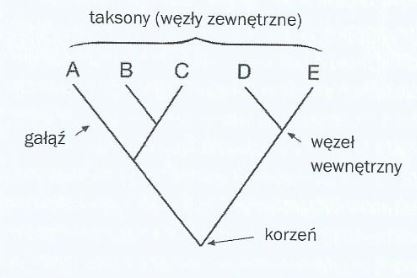
\includegraphics[width=0.55\textwidth]{typoweDrzewo}
	\caption{Typowe drzewo filogenetyczne \cite{1}}\label{Rysunek_typoweDrzewoFilogenetyczne}
\end{figure}

Ga��zie drzewa s� u�o�one wed�ug jego topologii. Ich podzia� na~dwie ga��zie potomne okre�la si� jako dychotomia (rys. \ref{Rysunek_dychotomiaIPolitomia}). Czasem wyst�puje tak�e politomia, czyli sytuacja, gdy z~punktu rozga��zienia odchodz� wi�cej ni� dwie ga��zie pochodne. Mo�e ona by� spowodowana tym, �e przodek da� jednocze�nie pocz�tek wi�cej ni� dw�m potomkom (tzw. proces radiacji) albo brakiem mo�liwo�ci precyzyjnego okre�lenia kolejno�ci podzia��w - niepe�nego rozwi�zania filogenezy.

\begin{figure}[!htb]
	\centering
	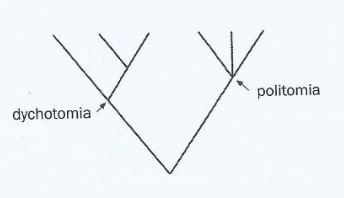
\includegraphics[width=0.65\textwidth]{dychotomiaIPolitomia2}
	\caption{Przyk�ad wyst�pienia dychotomii i politomii \cite{1}}\label{Rysunek_dychotomiaIPolitomia}
\end{figure}

\newpage
Istnieje mo�liwo�� konstruowania drzew ukorzenionych (rys. \ref{Rysunek_ukorzenienieDrzewa:c1}) - zak�adaj�cych znajomo�� wsp�lnego przodka - a tak�e nieukorzenionych (rys. \ref{Rysunek_ukorzenienieDrzewa:c2}), kt�re wy��cznie porz�dkuj� taksony zgodnie z~ich wzajemnymi powi�zaniami.
W celu ustalenia kierunku drogi ewolucyjnej, konieczne jest ukorzenienie drzewa \cite{1}.

\begin{figure}[H]
 \subfloat[Drzewo ukorzenione\label{Rysunek_ukorzenienieDrzewa:c1}]{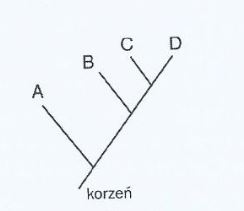
\includegraphics[width=0.4\textwidth]{drzewoUkorzenione2}} \; % <--- to daje odst�p w poziomie; \\ daje now� linijk�
 \subfloat[Drzewo nieukorzenione\label{Rysunek_ukorzenienieDrzewa:c2}]{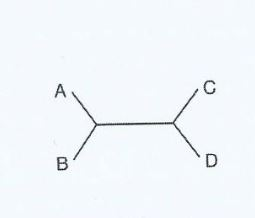
\includegraphics[width=0.4\textwidth]{drzewoNieukorzenione2}} 
  \caption{Por�wnanie drzewa ukorzenionego i nieukorzenionego \cite{1}\label{Rysunek_ukorzenienieDrzewa}} % wykorzystanie subref mo�e wymaga� dodania \protect !!!
\end{figure}

\subsection{Formy reprezentacji drzew} \label{formy_reprezentacji_drzew}
Jednym ze~sposob�w reprezentacji graficznej drzewa s� filogramy (\ref{filogram:c2}), gdzie d�ugo�� ga��zi zale�na jest od stopnia dywergencji ewolucyjnej. S� to drzewa wyskalowane. Prezentuj� one informacje, nie~tylko na~temat wyst�puj�cych zale�no�ci, ale te� o~ wzgl�dnym czasie dywergencji poszczeg�lnych ga��zi. W~przypadku drzew niewyskalowanych, wszystkie ga��zie s� jednakowej d�ugo�ci, co powoduje utrat� cz�ci informacji. Takie drzewa nazywa si� kladogramami \cite{1,2} (rys. \ref{kladogram:c1}).

\begin{figure}[H]
 \subfloat[Kladogram\label{kladogram:c1}]{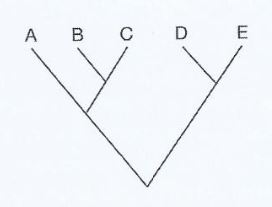
\includegraphics[width=0.4\textwidth]{kladogram}} \; % <--- to daje odst�p w poziomie; \\ daje now� linijk�
 \subfloat[Filogram\label{filogram:c2}]{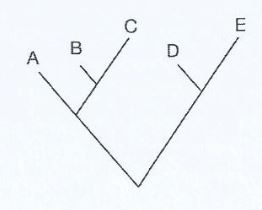
\includegraphics[width=0.4\textwidth]{filogram}} 
  \caption{Przyk�adowy kladogram i filogram \cite{1}\label{Rysunek_kladogram_i_filogram}} % wykorzystanie subref mo�e wymaga� dodania \protect !!!
\end{figure}

%\begin{figure}[!htb]
%	\centering
%	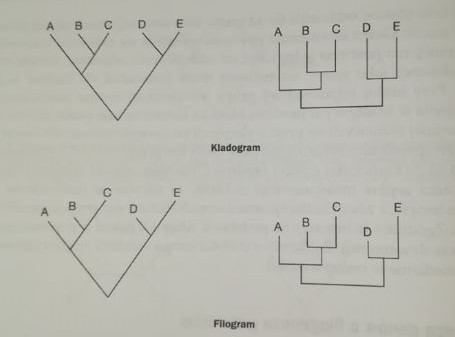
\includegraphics[width=0.65\textwidth]{kladogramyIFilogramyZ}
%	\caption{Przyk�adowe kladogramy i filogramy \cite{1}}\label{Rysunek_kladogramyIFilogramy}
%\end{figure}

\newpage
W celu przekazania opisu topologii drzewa do program�w komputerowych stosuje si� specjalny format tekstowy - Newick (rys. \ref{Rysunek_formatNewick}).

\begin{figure}[!htb]
	\centering
	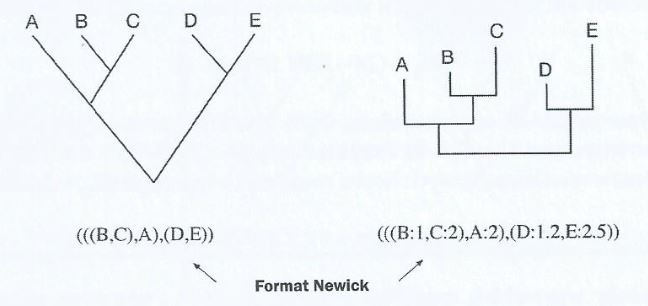
\includegraphics[width=0.75\textwidth]{formatNewick2}
	\caption{Przyk�ad zapisu drzew w~formacie Newick \cite{1}}\label{Rysunek_formatNewick}
\end{figure}

\subsection{Problemy w~szukaniu poprawnego drzewa}
Do poprawnej konstrukcji drzewa filogenetycznego niezb�dne jest znalezienie jego topologii i d�ugo�ci ga��zi, co nierzadko jest zadaniem trudnym i z�o�onym obliczeniowo. Liczba topologii drzewa mo�e by� bardzo du�a ju� przy~niewielkiej ilo�ci takson�w. Ro�nie ona wyk�adniczo zgodnie z~zale�no�ciami:
\begin{itemize}
 \item drzewa ukorzenione:
 \begin{equation}
 N_{R} = \dfrac{(2n-3)!}{2^{n-2}(n-2)!},
 \end{equation}
 \item drzewa nieukorzenione:
 \begin{equation}
 N_{U} = \dfrac{(2n-5)!}{2^{n-3}(n-3)!}.
 \end{equation}
\end{itemize}
			
\section{Etapy konstrukcji drzew filogenetycznych}
Podczas konstruowania drzew odwzorowuj�cych histori� ewolucji gatunk�w,
nale�y	uwzgl�dni� nast�puj�ce etapy:
\begin{itemize}
 \item wyb�r marker�w molekularnych - dane z~sekwencji nukleotydowych lub bia�kowych,
 \item przyr�wnanie sekwencji,
 \item wyb�r modelu ewolucji,
 \item wyb�r metody budowy drzewa,
 \item ocena wiarygodno�ci uzyskanego drzewa.
\end{itemize}
G��wnym za�o�eniem niniejszej pracy jest przeprowadzenie etapu czwartego - wyboru metody konstrukcji drzewa oraz zaprezentowanie jej przy~pomocy aplikacji.

\subsection{Mutacje i luki w~sekwencjach} \label{mutacje_i_luki}
Dobrym sposobem identyfikacji mutacji, kt�re wyst�pi�y podczas ewolucji i spowodowa�y rozbie�no�� sekwencji dw�ch badanych bia�ek jest dopasowanie sekwencji parami.
Najcz�ciej wyst�puj�ce mutacje to substytucje, insercje i delecje. W~sekwencjach bia�kowych substytucje wyst�puj�, gdy mutacja skutkuje zamian� kodonu dla jednego aminokwasu na~inny. Powoduje to dopasowanie dw�ch nieidentycznych aminokwas�w. Insercje i delecje wyst�puj�, gdy reszty s� dodawane lub usuwane. Zwykle s� one reprezentowane przez znak ,,-'' dodawany do jednej lub drugiej sekwencji.
 Insercje lub delecje (nawet te o~d�ugo�ci tylko jednego znaku) s� nazywane lukami w~wyr�wnaniu. Luki te mog� wyst�pi� na~ko�cu bia�ka lub w~�rodku. Jednym ze~skutk�w dodawania przerw jest spowodowanie, �e ca�kowita d�ugo�� ka�dego wyr�wnania jest taka sama. Dodanie luk mo�e pom�c w~stworzeniu dopasowania odwzorowuj�cego ewolucyjne zmiany, kt�re mia�y miejsce \cite{2}.

\subsection{Przyr�wnanie wielu sekwencji} \label{przyrownanie_wielu_sekwencji}
Przyr�wnanie wielu sekwencji jest zbiorem trzech lub wi�kszej liczby sekwencji bia�ka (lub kwasu nukleinowego), kt�re s� cz�ciowo lub ca�kowicie wyr�wnane. Homologiczne reszty s� wyr�wnane w~kolumnach na~ca�ej d�ugo�ci sekwencji. S� one homologiczne w~sensie ewolucyjnym - prawdopodobnie pochodz� od wsp�lnego przodka - oraz strukturalnym - wyr�wnane reszty maj� tendencj� do zajmowania odpowiednich pozycji w~tr�jwymiarowej strukturze ka�dego wyr�wnanego bia�ka. \cite{2}
Dopasowania wielu sekwencji nie~s� trudne do wygenerowania dla grupy bardzo blisko spokrewnionych sekwencji bia�kowych (lub DNA). Gdy tylko sekwencje wykazuj� pewn� rozbie�no��, problem wielokrotnego wyr�wnania staje si� niezwykle trudny do rozwi�zania. W~szczeg�lno�ci trudno jest oceni� liczb� i lokalizacj� luk. \cite{2}

\subsection{Modele substytucji} \label{model_Jukesa_Cantora}
Modele ewolucji kwas�w nukleinowych i bia�ek s� wykorzystywane w~metodach filogenetycznych jako podstawa do okre�lenia odleg�o�ci ewolucyjnych \cite{3}. Istnieje kilka modeli substytucji, kt�re s� ograniczone pod tym wzgl�dem, �e w~sytuacji, gdy na~danej pozycji wyst�pi zbyt wiele substytucji, dana pozycja zostaje wysycona. Oznacza to, �e dywergencja ewolucyjna przekracza mo�liwo�ci modeli do korekty homoplazji, a rzeczywiste odleg�o�ci ewolucyjne nie~s� mo�liwe do ustalenia \cite{1}.
Najprostszym modelem substytucji jest model Jukesa-Cantora (JC). Model opisuje jedno miejsce w~dopasowaniu sekwencji DNA. Podstaw� w~tym miejscu mo�e by� A, C, G lub T. Model zak�ada, �e wszystkie cztery zasady maj� jednakow� cz�stotliwo�� i �e istnieje szybko�� podstawienia $\alpha$ z~dowolnej z~czterech zasad DNA do dowolnej innej zasady. Liczba miejsc, kt�re r�ni� si� mi�dzy dwiema sekwencjami D jest bezpo�rednio obserwowalna przez por�wnanie dw�ch sekwencji, ale nie~uwzgl�dnia ona wszystkich zmian, kt�re zasz�y, poniewa� mog�o by� wi�cej ni� jedno podstawienie na~miejsce. Dlatego nale�y obliczy� ewolucyjn� odleg�o�� d, zdefiniowan� jako szacowana liczba substytucji, kt�re wyst�pi�y na~miejscu. \cite{3}
Zgodnie z~modelem Jukesa-Cantora odleg�o�� t� okre�la wz�r:
 \begin{equation}
 d_{AB} = -\frac{3}{4}ln[1 - \frac{4}{3}p_{AB}].
 \end{equation}

\subsection{Metody budowy drzew filogenetycznych}
Drzewa mo�na tworzy� przy~pomocy metod nale��cych do dw�ch kategorii:
\begin{itemize}
 \item metody oparte na~odleg�o�ciach:
 \begin{itemize}
  \item [-] klasteryzacja, np. metoda grupowania niewa�onych par z~arytmetycznymi �rednimi (UPGMA), metoda ��czenia s�siad�w (metoda najbli�szego s�siedztwa - NJ), uog�lniona metoda NJ,
  \item [-] kryterium optymalno�ci, np. metoda Fitcha-Margoliasha (FM), metoda minimalnej ewolucji (ME);
 \end{itemize}
 \item metody oparte na~znakach sekwencji takson�w:
 \begin{itemize}
  \item [-] metoda maksymalnej parsymonii (MP), wa�ona parsymonia, metoda kwarter�w, metoda najwi�kszej wiarygodno�ci (ML), metoda NJML (po��czenie metod NJ i ML), algorytm genetyczny (GA).
 \end{itemize}
\end{itemize}

\subsection{Por�wnanie metod UPGMA i WPGMA} \label{UPGMA_WPGMA}
Zar�wno metoda UPGMA, jak i WPGMA to metody klastrowania.W metodzie UPGMA odleg�o�� mi�dzy dwoma klastrami jest �redni� odleg�o�ci� mi�dzy wszystkimi obiektami ka�dego klastra, natomiast w~metodzie WPGMA odleg�o�� mi�dzy dwoma klastrami jest �redni� arytmetyczn� odleg�o�ci mi�dzy obiektami ka�dego klastra wa�on� przez liczb� obiekt�w w~ka�dym klastrze \cite{4}.
Algorytm obydwu metod:
\begin{itemize}
\item znajd� warto�� minimaln� (dwie najmniej r�ni�ce si�/najbli�sze sekwencje) macierzy odleg�o�ci ewolucyjnych,
\item po��cz najbli�sze sekwencje tworz�c klaster,
\item oblicz now� macierz odleg�o�ci ewolucyjnych:
\begin{itemize}
\item[-]UPGMA - oblicz �redni� arytmetyczn� bior�c pod uwag� wszystkie sekwencje nale��ce do tworzonego klastera,
\item[-]WPGMA - oblicz �redni� arytmetyczn� bior�c pod uwag� dwa klastery tworz�ce nowy klaster.
\end{itemize}
\item powtarzaj, dop�ki nie~zostan� po��czone wszystkie sekwencje.
\end{itemize}

Na rysunku \ref{Rysunek_UPGMA_vs_WPGMA} por�wnano wygl�d przyk�adowej macierzy odleg�o�ci ewolucyjnych w~kolejnych krokach dla metody UPGMA i WPGMA \cite{5, 6}.

\begin{figure}[H]
 \subfloat[Metoda UPGMA etap I\label{Rysunek_UPGMA_etap1:c1}]{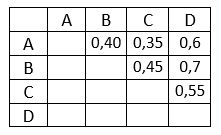
\includegraphics[width=0.4\textwidth]{macierz1}} \; 
 \subfloat[Metoda WPGMA etap I\label{Rysunek_WPGMA_etap1:c2}]{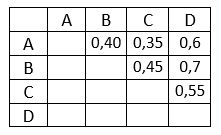
\includegraphics[width=0.4\textwidth]{macierz1}} \;
 \subfloat[Metoda UPGMA etap II\label{Rysunek_UPGMA_etap2:c2}]{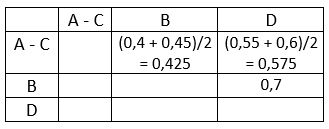
\includegraphics[width=0.5\textwidth]{macierz2}} \;
 \subfloat[Metoda WPGMA etap II\label{Rysunek_WPGMA_etap2:c2}]{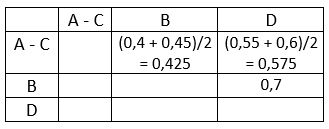
\includegraphics[width=0.5\textwidth]{macierz2}} \;
 \subfloat[Metoda WPGMA etap III\label{Rysunek_UPGMA_etap3:c2}]{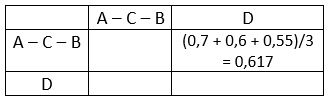
\includegraphics[width=0.5\textwidth]{macierz3U}} \;
\subfloat[Metoda WPGMA etap III\label{Rysunek_UPGMA_etap3:c2}]{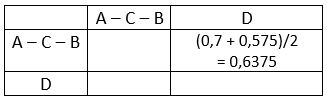
\includegraphics[width=0.5\textwidth]{macierz3W}}  
  \caption{Por�wnanie kolejnych etap�w w~metodzie UPGMA i WPGMA\label{Rysunek_UPGMA_vs_WPGMA}}
\end{figure}


\section{Metodologia} \label{mteodologia}
Problem przedstawiony w~projekcie to konstrukcja drzew filogenetycznych. Jako jego rozwi�zanie zaproponowano program, przyjmuj�cy na~wej�ciu fragmenty sekwencji nukleotydowych, kt�re zostaj� przyr�wnane (\ref{przyrownanie_wielu_sekwencji}). Efektem jest macierz odleg�o�ci ewolucyjnych zawieraj�ca wyniki (odleg�o�ci ewolucyjne) dla ka�dej pary sekwencji. Uzyskuje si� je przy~pomocy modelu substytucji Jukesa - Cantora (\ref{model_Jukesa_Cantora}). Nast�pnie, na~podstawie wy�ej wymienionej macierzy i zgodnie z~metod� WPGMA (\ref {UPGMA_WPGMA}) tworzone s� drzewa filogenetyczne dla danych sekwencji. Graficznie przedstawiane s� jako kladogramy (\ref{formy_reprezentacji_drzew}), jednak informacja o~d�ugo�ci poszczeg�lnych ga��zi drzewa nie~jest zatracana, lecz przedstawiona w~formie kolejnej macierzy.

%schemat blokowy?

\chapter{Specyfikacja wewn�trzna}
Aplikacj� zaimplementowano w~�rodowisku Matlab, z~powodu wzgl�dnie prostego sposobu operowania na macierzach i~graficznej prezentacji drzew binarnych.
Nazwa programu, podobnie jak~jej~g��wnej funkcji to~\textit{FilogeneticTrees}. W~celu u�atwienia korzystania z~aplikacji, utworzono graficzny interfejs u�ytkownika, r�wnie� o~tej~samej nazwie.
\newline
Jak~wspomniano (\ref{mteodologia}), parametrem przyjmowanym na~wej�ciu s�~fragmenty sekwencji nukleotydowych jako~�a�cuchy znak�w. Mo�liwe jest~zatem wpisanie liter: ,,A'', ,,G", ,,C'', ,,T'' oraz oznaczaj�cego luk� w~sekwencji, ,,-''. Program nie~przyjmuje innych znak�w, co~zosta�o zapewnione funkcj� \textit{checkIfThereIsNoIllegalSign}.
\newline
Kolejnym krokiem jest~przyr�wnanie wielu sekwencji (\ref{przyrownanie_wielu_sekwencji}). Odpowiada za~nie~funkcja \textit{compareSequences}. Por�wnywane sekwencje powinny by�~takiej samej d�ugo�ci, nie~powinny by�~identyczne, ani~r�ni� si�~bardziej ni�~w~75\%. Aby~zabezpieczy� program przed~przerwaniem jego~dzia�ania w~wymienionych przypadkach, utworzono funkcje, odpowiednio \textit{checkIfLengthIsEqual} i~\textit{checkTheDifferencesBetweenSequences}. Je�li~wszystkie warunki zosta�y spe�nione, przy~pomocy funkcji \textit{makeMatrixOfSequences} tworzona jest~macierz, w~kt�rej znajduj� si�~wszystkie podane sekwencje (pomini�te zostaj� pola tekstowe, kt�re u�ytkownik pozostawi� puste). Funkcja zwraca tak�e d�ugo�� sekwencji potrzebn� w~dalszych obliczeniach. Nast�puje te�~w�a�ciwe por�wnywanie sekwencji, kt�rego efektem jest~powstanie macierzy odleg�o�ci ewolucyjnych. Umieszczone w~niej warto�ci to~odleg�o�ci (ilo�ci znak�w r�ni�cych si�) pomi�dzy sekwencjami po~zastosowaniu modelu substytucji Jukesa-Cantora (\ref{model_Jukesa_Cantora}) przy~u�yciu funkcji \textit{jukesCantorSubstituteModel}.
\newline
Podczas przyr�wnywania sekwencji, w~programie g��wnym zostaje wywo�ana funkcja \textit{createTreeByWpgmaMethod} jako~argument przyjmuj�ca utworzon� wcze�niej macierz odleg�o�ci ewolucyjnych. Wewn�trz niej zosta� zawarty kod umo�liwiaj�cy otrzymanie ko�cowej postaci drzewa filogenetycznego metod� WPGMA, a~tak�e parametr�w koniecznych do~jego graficznego zaprezentowania. U�yto tu~takich funkcji, jak:
\begin{itemize}
\item \textit{findFirstMinimumPosition} - odpowiedzialn� za~wyszukanie minimalnej warto�ci macierzy odleg�o�ci ewolucyjnych, czyli zdefiniowanie, kt�re sekwencje lub~klastery s�~sobie najbli�sze (ewolucyjnie), a~co~za~tym~idzie - nale�y po��czy� w~danej iteracji,
\item \textit{calculateBranchLength} - zwracaj�c� d�ugo�� ga��zi drzewa w~danej iteracji (jest~to po�owa odnalezionej minimalnej warto�ci odleg�o�ci); zwracana warto�� zostaje dopisana do~wektora d�ugo�ci ga��zi \textit{branchLengthVector}, by~pos�u�y� do~obliczenia ostatecznych odleg�o�ci pomi�dzy sekwencjami,
\item \textit{makeClusterGroups} - przy~jej pomocy tworzone s�~odpowiednie klastery lub do~ju�~istniej�cych do��czane s�~nowe sekwencje; jest~to~mo�liwe, mi�dzy innymi dzi�ki funkcji \textit{mergeRows}, kt�ra s�u�y do~��czenia dw�ch istniej�cych klaster�w, czyli kiedy nie~jest~do��czana �adna nowa sekwencja; w~programie zrealizowano to~jako~po��czenie dw�ch wierszy macierzy klastr�w \textit{clusterGroupsArray},
\item \textit{makeHelperClusterVectors} - za~pomoc� dw�ch wektor�w okre�laj�c�, kt�re sekwencje nie~zosta�y jeszcze do��czone do~tworzonego drzewa,
\item \textit{calculateNewDistanceMatrix} - tworz�c�, na~podstawie obecnych danych i~pozycji warto�ci minimalnej, now� posta� macierzy odleg�o�ci ewolucyjnych, zgodnie z~metod� WPGMA dla~kolejnych iteracji,
\item \textit{calculateParametersToDrawTree} - definiuj�c� takie parametry, jak~liczba w�z��w drzewa \textit{nodesNumber}, wektor w�z��w okre�laj�cy ich~po�o�enie wzgl�dem siebie \textit{nodes} czy~wskazuj�c�, kt�re z~w�z��w powinny zosta� oznaczone jako~,,li�cie'' drzewa, czyli sekwencje.
\end{itemize}
Aplikacja umo�liwia u�ytkownikowi wgl�d w~warto�ci macierzy odleg�o�ci ewolucyjnych oraz~przedstawia aktualny wygl�d tworzonego drzewa filogenetycznego dla~ka�dej iteracji. Zrealizowano to~za~pomoc� wy�ej wymienionego rozwi�zania (kolejne postaci macierzy) oraz~funkcji \textit{displayTree} przyjmuj�cej obliczone parametry i~wy�wietlaj�cej obecn� cz�� drzewa. 
\newline
Ostatni� z~wykorzystanych funkcji jest~\textit{signLeafsAsSequencesNumbers}, kt�ra pozwala na~w�a�ciwe podpisanie w�z��w drzewa jako~sekwencji.

\chapter{Specyfikacja zewn�trzna}
Program zosta� zaimplementowany w~wersji Matlab R2015a. W~celu korzystania z~aplikacji, nale�y uruchomi� plik \textit{FilogeneticTrees.m} przyciskaj�c przycisk \textbf{,,Run''} (rys. \ref{Rysunek_run}).

\begin{figure}[!htb]
	\centering
	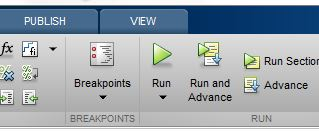
\includegraphics[width=0.55\textwidth]{runForrestRun}
	\caption{Uruchamianie aplikacji}\label{Rysunek_run}
\end{figure}

Spowoduje to pojawienie si� g��wnego okna aplikacji (rys. \ref{Rysunek_appMainWin}), gdzie nast�pnie nale�y wpisa� w odpowiednie pola fragmenty kolejnych, przyr�wnywanych sekwencji nukleotydowych (nr 1 na rys. \ref{Rysunek_appMainWin}), np. \textbf{AGCTGTGA}.

\begin{figure}[!htb]
	\centering
	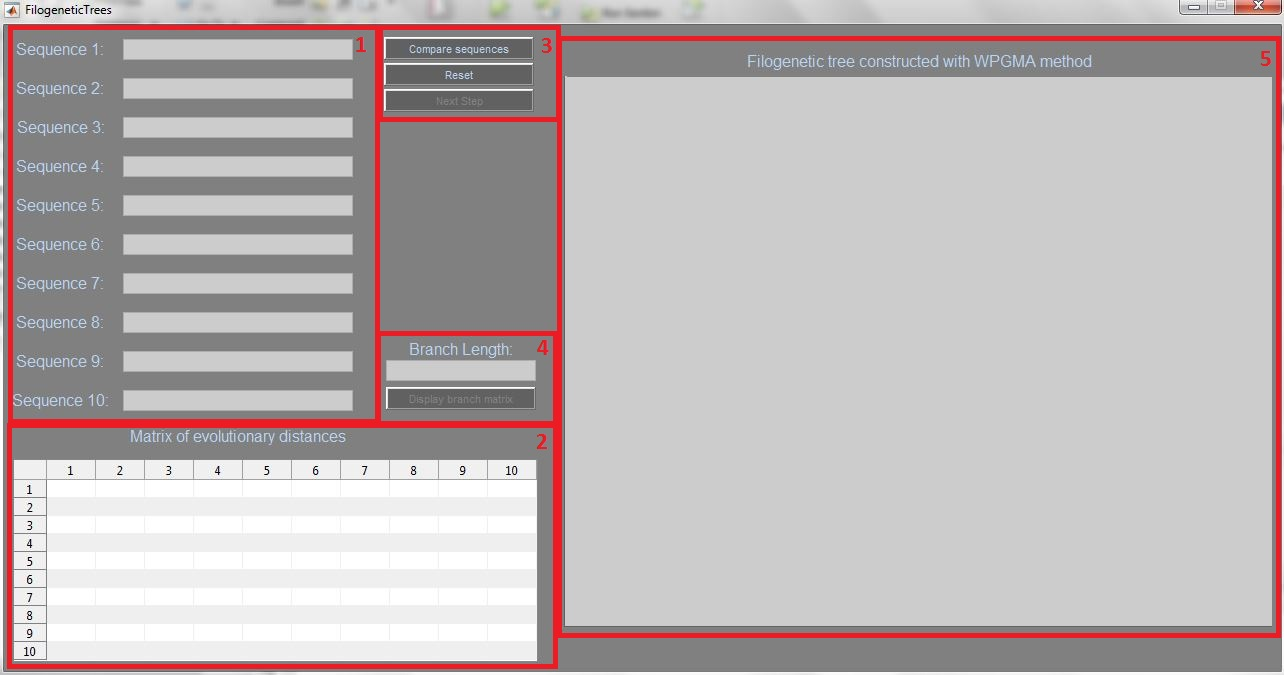
\includegraphics[width=1\textwidth]{appMainWinNum}
	\caption{G��wne okno aplikacji}\label{Rysunek_appMainWin}
\end{figure}

Sekwencje nie mog� si� powtarza�, ani r�ni� od siebie w ponad 75\% (jest to zwi�zane z wykorzystaniem modelu substytucji Jukesa-Cantora i wiarygodno�ci� wykonywanych oblicze�). Je�li te warunki nie b�d� spe�nione, aplikacja wy�wietli komunikat o b��dzie (rys. \ref{Rysunek_differenceErrors}). Konieczne jest wpisanie co najmniej dw�ch sekwencji, w przeciwnym razie program nie wykona �adnych oblicze� i wy�wietli ostrze�enie (rys. \ref{Rysunek_atLeastTwoError:c2}).

\begin{figure}[H]
 \subfloat[B��d powt�rzonej sekwencji\label{Rysunek_theSameError:c1}]{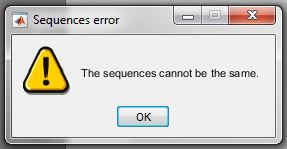
\includegraphics[width=0.4\textwidth]{theSameError}} \;
 \subfloat[B��d zbyt du�ej r�nicy mi�dzy sekwencjami\label{Rysunek_differenceError:c2}]{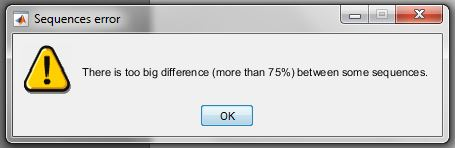
\includegraphics[width=0.6\textwidth]{differenceError}}  \;
  \subfloat[Ostrze�enie o zbyt ma�ej liczbie wpisanych sekwencji\label{Rysunek_atLeastTwoError:c2}]{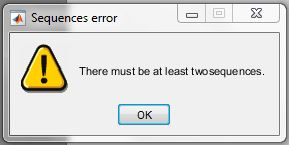
\includegraphics[width=0.5\textwidth]{atLeastTwoError}} 
  \caption{Komunikaty o b��dach dotycz�cych zawarto�ci wpisanych sekwencji \label{Rysunek_differenceErrors}}
\end{figure}

 R�wnie� w przypadku r�nych d�ugo�ci sekwencji lub wpisania niedozwolonego znaku (innego ni� ,,A'', ,,G'', ,,C'', ,,T'' lub ,,-'') u�ytkownik zostaje o tym poinformowany (rys. \ref{Rysunek_lengthIllegalErrors}).
 
\begin{figure}[H]
 \subfloat[B��d r�nych d�ugo�ci sekwencji\label{Rysunek_lengthError:c1}]{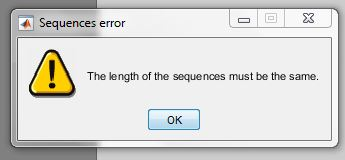
\includegraphics[width=0.45\textwidth]{lengthError}} \;
 \subfloat[B��d niedozwolonych znak�w w sekwencji \label{Rysunek_illegalSignError:c2}]{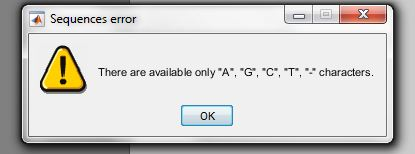
\includegraphics[width=0.55\textwidth]{illegalSignError}} 
  \caption{Komunikaty o b��dach dotycz�cych d�ugo�ci i znak�w w sekwencjach \label{Rysunek_lengthIllegalErrors}}
\end{figure}
 
 Po upewnieniu si�, �e podane sekwencje maj� w�a�ciwy format nale�y wcisn�� przycisk \textbf{,,Compare sequences''} (nr 3 na rys. \ref{Rysunek_appMainWin}). Skutkuje to:
 \begin{itemize}
 \item zablokowaniem wy�ej wymienionego przycisku,
 \item zablokowaniem p�l tekstowych,
 \item odblokowaniem przycisku \textbf{,,Next step''} oraz wy�wietleniem obliczonych warto�ci pocz�tkowej macierzy odleg�o�ci ewolucyjnych (nr 2 na rys. \ref{Rysunek_appMainWin}) lub - w przypadku wyst�pienia b��du - pojawieniem si� komunikatu (rys. \ref{Rysunek_afterCompareBtns}).
 \end{itemize} 
 
\begin{figure}[H]
 \subfloat[Efekt wci�ni�cia przycisku \textbf{,,Compare sequenses''} w przypadku prawid�owego dzia�ania \label{Rysunek_afterCompareBtn:c1}]{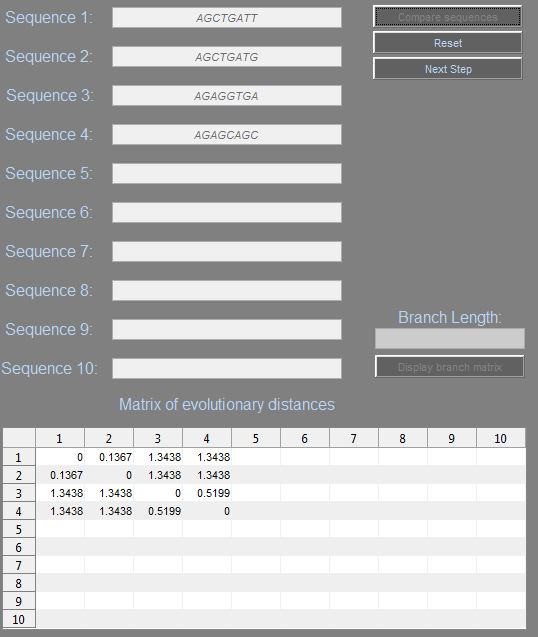
\includegraphics[width=0.55\textwidth]{afterCompareBtn}} \;
 \subfloat[Efekt wci�ni�cia przycisku \textbf{,,Compare sequenses''} w przypadku wyst�pienia b��du \label{Rysunek_afterCompareBtnError:c2}]{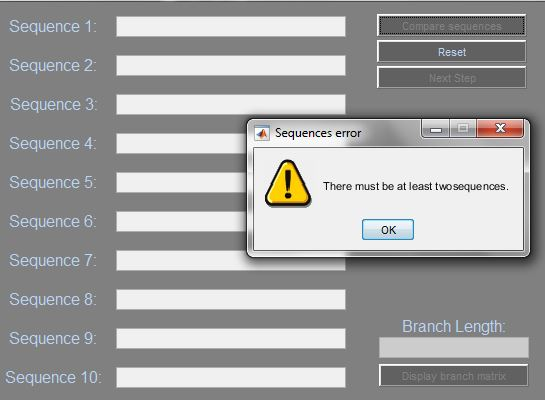
\includegraphics[width=0.55\textwidth]{afterCompareBtnError}} 
  \caption{Widok aplikacji po wci�ni�ciu przycisku \textbf{,,Compare sequences''} \label{Rysunek_afterCompareBtns}}
\end{figure}

Kolejn� czynno�ci� jest wywo�anie nast�pnego kroku w tworzeniu drzewa filogenetycznego przy u�yciu przycisku \textbf{,,Next step''}. W efekcie obliczona zostaje nowa macierz odleg�o�ci ewolucyjnych (o rozmiarze o 1 mniejszym w stosunku do poprzedniego kroku) i wpisana na miejsce starej. Wy�wietlone zostaje tak�e poddrzewo ko�cowego drzewa filogenetycznego, w specjalnie wyznaczonym oknie (nr 5 na rys. \ref{Rysunek_appMainWin}), kt�re tworzone jest zgodnie z bie��cymi obliczeniami. 
\newpage
Dzi�ki temu u�ytkownik mo�e obserwowa� rozrost drzewa krok po kroku a� do uzyskania ko�cowego efektu (rys. \ref{Rysunek_afterNextStepBtn}). Dodatkowo, w polu tekstowym (nr 4 na rys. \ref{Rysunek_appMainWin}) wy�wietlana jest d�ugo�� bie��cej ga��zi drzewa.

\begin{figure}[!htb]
	\centering
	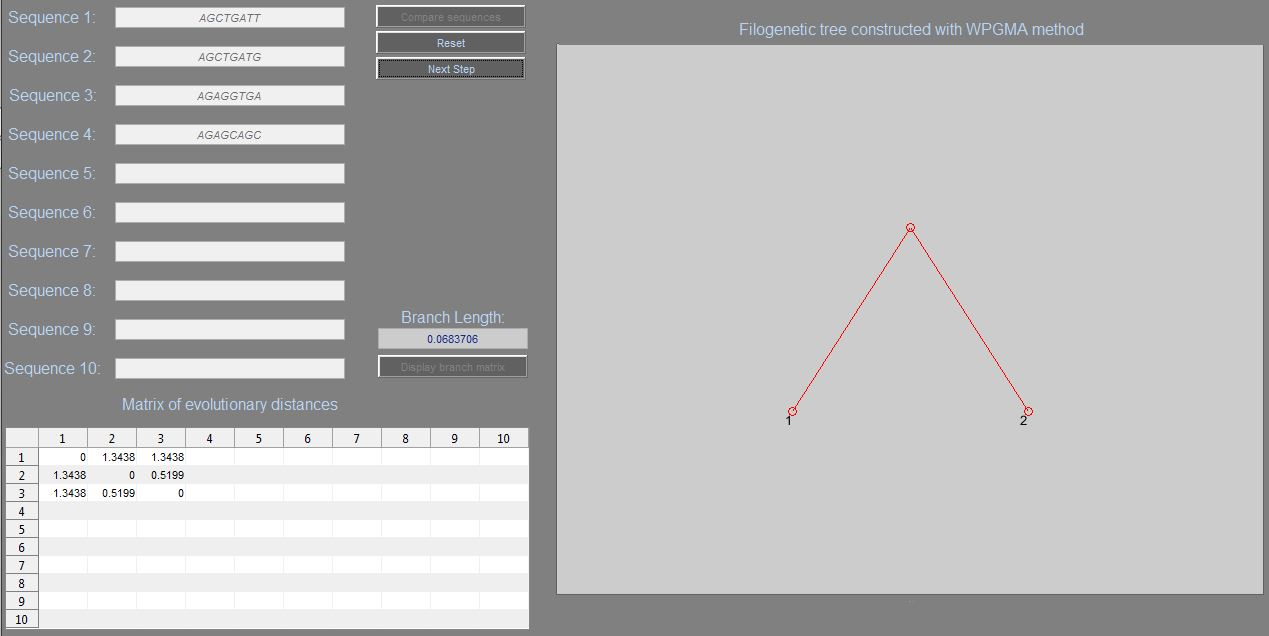
\includegraphics[width=1\textwidth]{afterNextStepBtn}
	\caption{Przyk�ad efektu dzia�ania przycisku \textbf{,,Next step''}}\label{Rysunek_afterNextStepBtn}
\end{figure}

Po przej�ciu do ostatniego kroku, zablokowany zostaje przycisk \textbf{,,Next step''}, natomiast mo�liwe jest u�ycie przycisku \textbf{,,Display branch matrix''} (rys. \ref{Rysunek_lastSteps}). 

\begin{figure}[!htb]
	\centering
	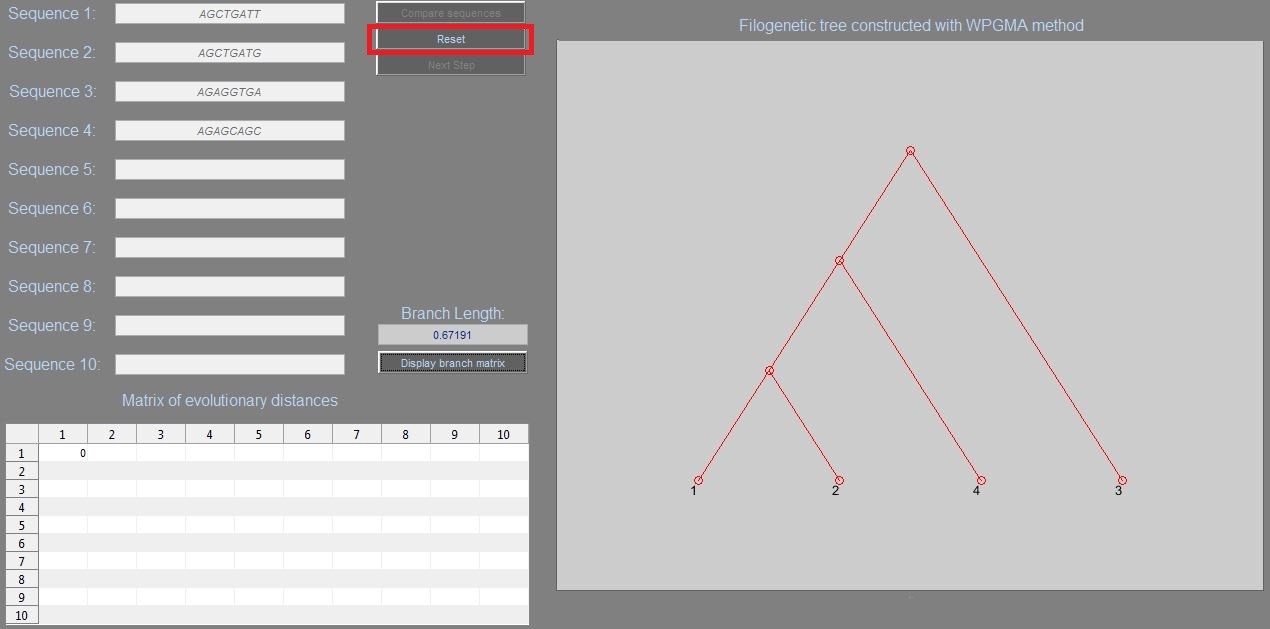
\includegraphics[width=1\textwidth]{lastStepss1}
	\caption{Wygl�d aplikacji po przej�ciu wszystkich krok�w tworzenia drzewa \label{Rysunek_lastSteps}}
\end{figure}

\newpage
Pozwala on na wy�wietlenie w osobnym oknie (rys. \ref{Rysunek_branchMatrix}) macierzy zawieraj�cej odleg�o�ci pomi�dzy wszystkimi sekwencjami. Warto�ci te obliczane s� na podstawie wcze�niej uzyskanych d�ugo�ci poszczeg�lnych ga��zi.

\begin{figure}[!htb]
	\centering
	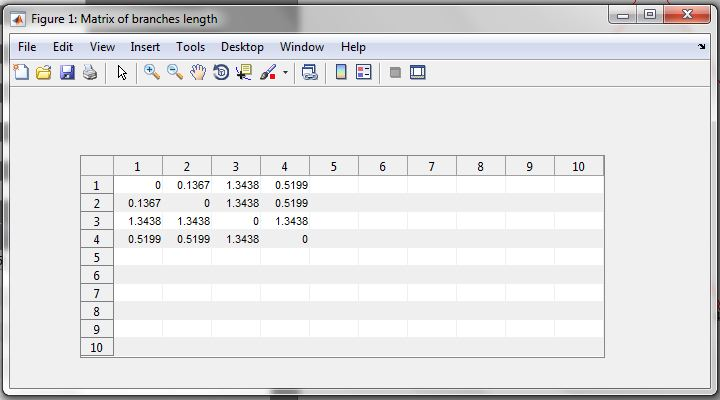
\includegraphics[width=0.8\textwidth]{branchMatrix}
	\caption{Przyk�adowa macierz odleg�o�ci pomi�dzy sekwencjami obliczonymi na podstawie d�ugo�ci ga��zi drzewa}\label{Rysunek_branchMatrix}
\end{figure}

W aplikacji uwzgl�dniono tak�e jej przywr�cenie do momentu wpisywania sekwencji. Aby to uczyni�, nale�y u�y� przycisku \textbf{,,Reset''} (zaznaczony na czerwono na rys. \ref{Rysunek_lastSteps}) dost�pnego przez ca�y czas dzia�ania programu.

\newpage
\section{Symulacja dzia�ania programu}
\subsection{Wprowadzenie danych}

Do symulacji u�yto fragment�w sze�ciu losowych sekwencji nukleotydowych (rys. \ref{Rysunek_samples1}).

\begin{figure}[!htb]
	\centering
	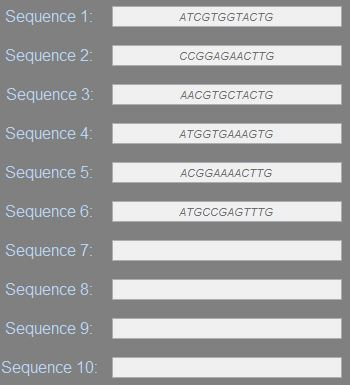
\includegraphics[width=0.5\textwidth]{samples1}
	\caption{Przyk�adowe sekwencje nukleotydowe}\label{Rysunek_samples1}
\end{figure}

Po u�yciu przycisku \textbf{,,Compare sequences''} zostaje obliczona pierwotna posta� macierzy odleg�o�ci ewolucyjnych (rys. \ref{Rysunek_matrix1}).

\begin{figure}[!htb]
	\centering
	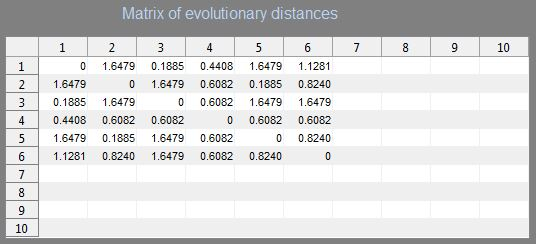
\includegraphics[width=0.7\textwidth]{matrix1}
	\caption{Pierwotna posta� macierzy odleg�o�ci ewolucyjnych}\label{Rysunek_matrix1}
\end{figure}

\subsection{Wyznaczanie kolejnych ga��zi drzewa}

Wykorzystuj�c przycisk \textbf{,,Next step''} uzyskano nowe warto�ci w macierzy odleg�o�ci ewolucyjnych, d�ugo�� ga��zi oraz grafik� przedstawiaj�c� drzewo w kolejnych etapach (rys. \ref{Rysunek_matrix2} - \ref{Rysunek_treePlace5}).

%\subsubsection{Krok pierwszy}
\begin{figure}[!htb]
	\centering
	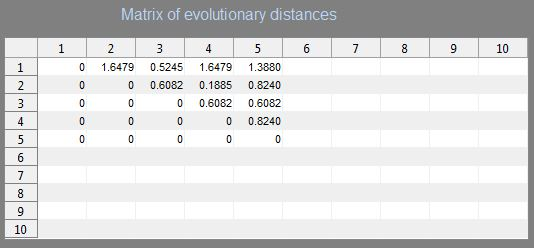
\includegraphics[width=0.7\textwidth]{matrix2}
	\caption{Pierwotna posta� macierzy odleg�o�ci ewolucyjnych}\label{Rysunek_matrix2}
\end{figure}

\begin{figure}[!htb]
	\centering
	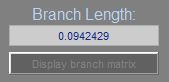
\includegraphics[width=0.2\textwidth]{branchLength1}
	\caption{D�ugo�� dw�ch pierwszych ga��zi drzewa}\label{Rysunek_branchLength1}
\end{figure}

\begin{figure}[!htb]
	\centering
	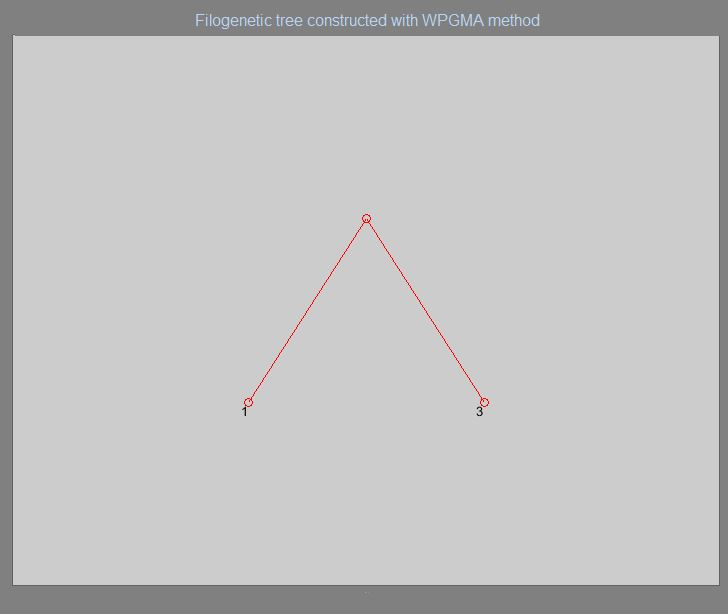
\includegraphics[width=0.65\textwidth]{treePlace1}
	\caption{Graficzne przedstawienie dw�ch pierwszych ga��zi drzewa}\label{Rysunek_treePlace1}
\end{figure}

\newpage
\subsubsection{Krok drugi}
\begin{figure}[!htb]
	\centering
	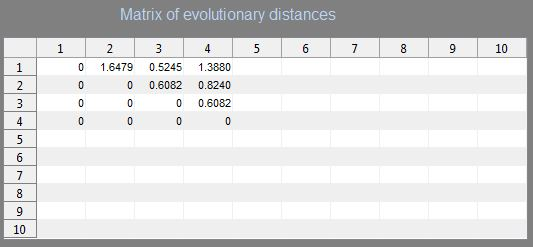
\includegraphics[width=0.7\textwidth]{matrix3}
	\caption{Macierz odleg�o�ci ewolucyjnych - krok drugi}\label{Rysunek_matrix3}
\end{figure}

\begin{figure}[!htb]
	\centering
	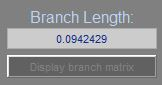
\includegraphics[width=0.2\textwidth]{branchLength2}
	\caption{D�ugo�� kolejnych dw�ch ga��zi drzewa - krok drugi}\label{Rysunek_branchLength2}
\end{figure}

\begin{figure}[!htb]
	\centering
	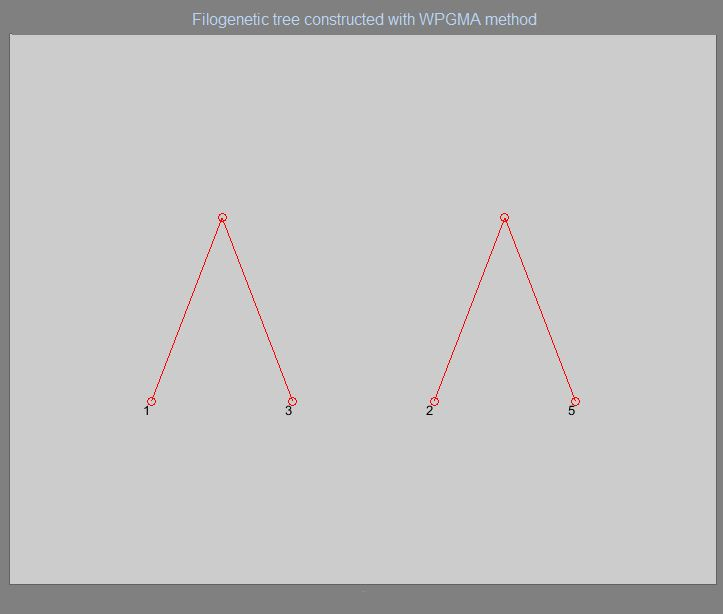
\includegraphics[width=0.65\textwidth]{treePlace2}
	\caption{Graficzne przedstawienie kolejnych dw�ch ga��zi drzewa - krok drugi}\label{Rysunek_treePlace2}
\end{figure}

\newpage
\subsubsection{Krok trzeci}
\begin{figure}[!htb]
	\centering
	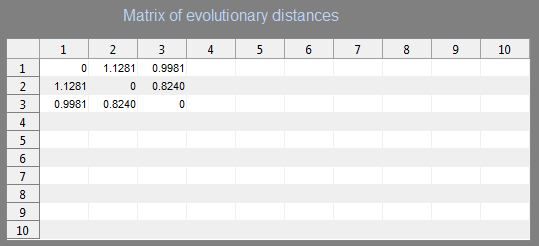
\includegraphics[width=0.7\textwidth]{matrix4}
	\caption{Macierz odleg�o�ci ewolucyjnych - krok trzeci}\label{Rysunek_matrix4}
\end{figure}

\begin{figure}[!htb]
	\centering
	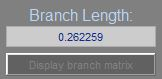
\includegraphics[width=0.2\textwidth]{branchLength3}
	\caption{D�ugo�� kolejnych dw�ch ga��zi drzewa - krok trzeci}\label{Rysunek_branchLength3}
\end{figure}

\begin{figure}[!htb]
	\centering
	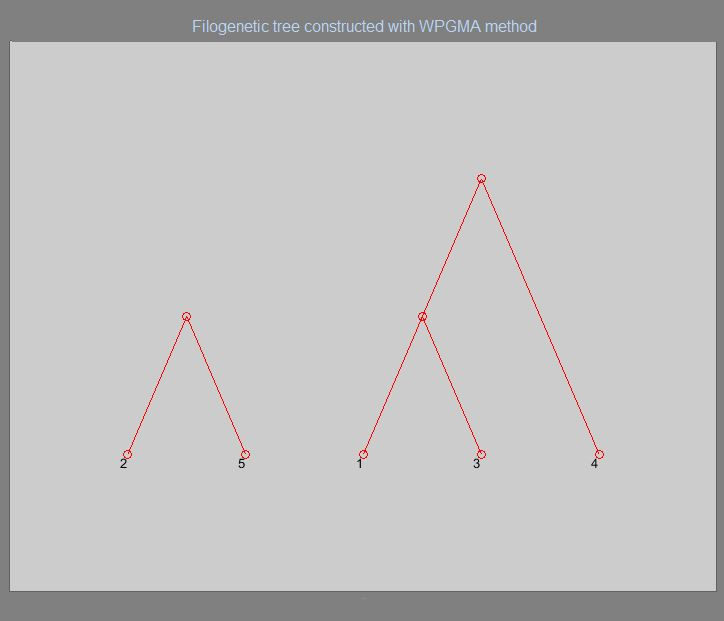
\includegraphics[width=0.65\textwidth]{treePlace3}
	\caption{Graficzne przedstawienie kolejnych dw�ch ga��zi drzewa - krok trzeci}\label{Rysunek_treePlace3}
\end{figure}

\newpage
\subsubsection{Krok czwarty}
\begin{figure}[!htb]
	\centering
	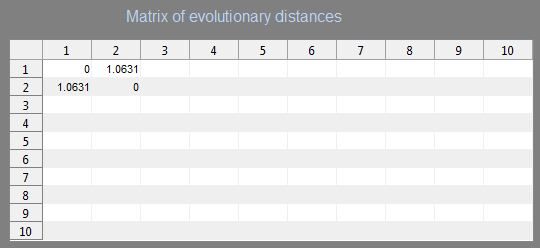
\includegraphics[width=0.7\textwidth]{matrix5}
	\caption{Macierz odleg�o�ci ewolucyjnych - krok czwarty}\label{Rysunek_matrix5}
\end{figure}

\begin{figure}[!htb]
	\centering
	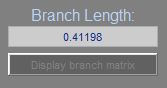
\includegraphics[width=0.2\textwidth]{branchLength4}
	\caption{D�ugo�� kolejnych dw�ch ga��zi drzewa - krok czwarty}\label{Rysunek_branchLength4}
\end{figure}

\begin{figure}[!htb]
	\centering
	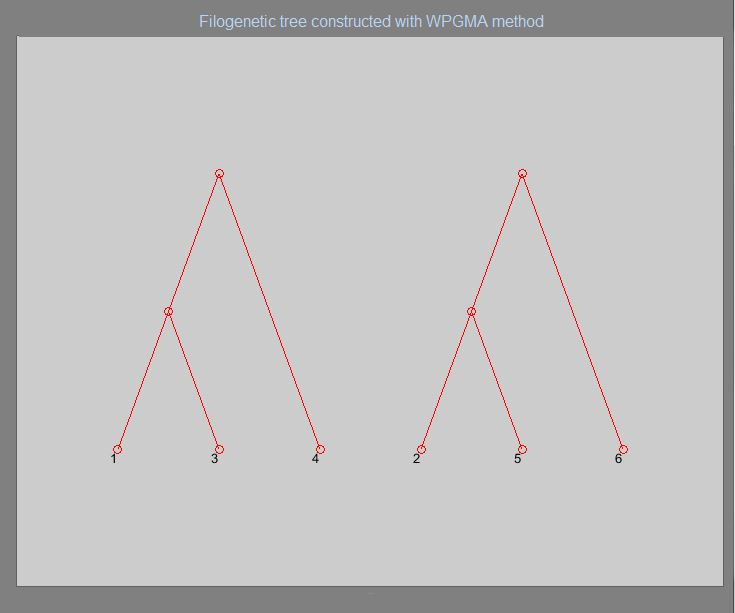
\includegraphics[width=0.65\textwidth]{treePlace4}
	\caption{Graficzne przedstawienie kolejnych dw�ch ga��zi drzewa - krok czwarty}\label{Rysunek_treePlace4}
\end{figure}

\newpage
\subsubsection{Krok pi�ty}
\begin{figure}[!htb]
	\centering
	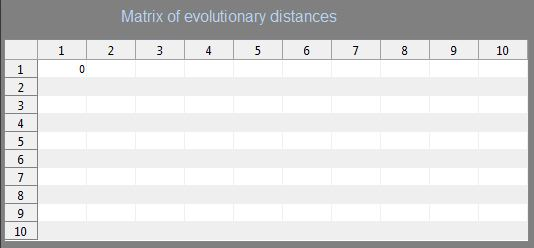
\includegraphics[width=0.7\textwidth]{matrix6}
	\caption{Macierz odleg�o�ci ewolucyjnych - krok pi�ty}\label{Rysunek_matrix6}
\end{figure}

\begin{figure}[!htb]
	\centering
	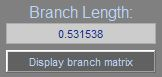
\includegraphics[width=0.2\textwidth]{branchLength5}
	\caption{D�ugo�� kolejnych dw�ch ga��zi drzewa - krok pi�ty}\label{Rysunek_branchLength5}
\end{figure}

\begin{figure}[!htb]
	\centering
	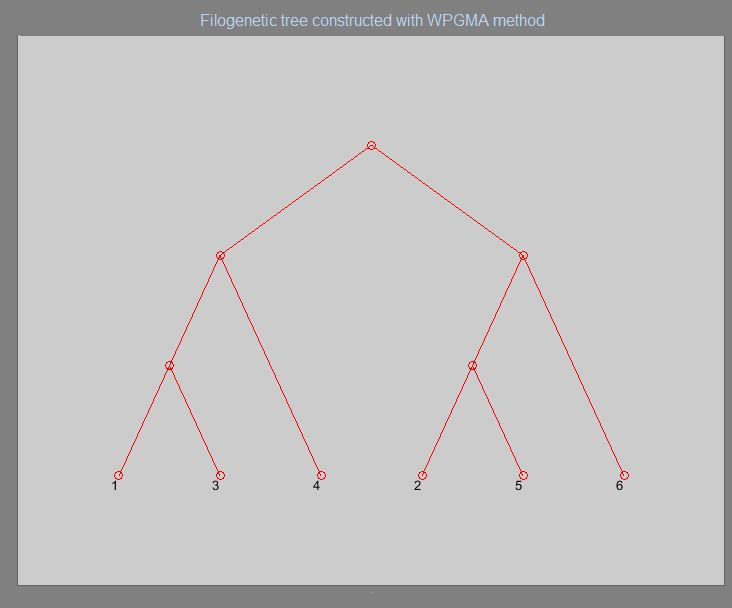
\includegraphics[width=0.65\textwidth]{treePlace5}
	\caption{Graficzne przedstawienie kolejnych dw�ch ga��zi drzewa - krok pi�ty}\label{Rysunek_treePlace5}
\end{figure}

\newpage
Po zako�czeniu oblicze�, przycisk \textbf{,,Next step''} zostaje zablokowany, natomiast mo�liwe staje si� u�ycie przycisku \textbf{,,Display branch matrix''}. Jego naci�ni�cie powoduje pojawienie si� nowego okna, w kt�rym przedstawiono macierz odleg�o�ci pomi�dzy sekwencjami obliczanych na podstawie wcze�niej uzyskanych d�ugo�ci poszczeg�lnych ga��zi.


%\chapter{Rezultaty}
%Zobrazowanie i om�wienie wynik�w otrzymywanych wskutek zastosowania danego urz�dzenia b�d� aplikacji. Badanie ewentualnych parametr�w (takich jak dok�adno��, czu�o��...), czy te� zachowania w szczeg�lnych sytuacjach. O ile to mo�liwe tabelaryzacja rezultat�w oraz ich statystyczna interpretacja. Ocena zachowania zaproponowanego rozwi�zania. Analiza mo�liwych przyczyn wyst�pienia b��d�w. 

%%%%%%%%%%%%%%%%%%%%%%%%%%%%%%%%%%%%%%%%%%%%%%%%%%%%%%%%%%%%%%%%%%%%%%%%%%%%%%%%%%%%%%%%%%%%%%%%%%%%%%%%%%%%%%%%%%%%%%%%%%%%%%%%%%%%%%%%%%%%%%%%%%%%%%%%%%%%%%%%%%%%%%%
%\chapter{Podsumowanie}
%Nawi�zanie do celu pracy oraz postawionych za�o�e�. Pr�ba oceny realizacji celu, poprzez weryfikacj� otrzymanych rezultat�w. Analiza dostrze�onych problem�w, b��dnego, nieoczekiwanego dzia�ania, ewentualnych problem�w napotkanych podczas realizacji. W przypadku niewyczerpania tematu, a tak�e wspomnianego niepo��danego zachowania urz�dzenia/aplikacji sugestie ich eliminacji wymienione jako plany na przysz�o��.\footnote{Kr�tkie! 1-2 strony.}
%
%Wst�p wraz z podsumowaniem winny stanowi� swego rodzaju klamr�, a nawet ca�o�� w takim rozumieniu, �e przeczytanie wy��cznie tych dw�ch rozdzia��w t�umaczy� powinno rozwa�any problem wraz z efektami otrzymanymi w efekcie prac, stanowi�cymi jego rozwi�zanie, bez wnikania w spos�b ich otrzymania (to zawiera cz�� �rodkowa).
%
\begin{thebibliography}{9}
\bibitem{1} Xiong J., ,,Podstawy bioinformatyki'', Wydawnictwa Uniwersytetu Warszawskiego, 2009, Warszawa
\bibitem{2} Pevsner J., ,,Bioinformatics and functional genomics'', third edition, Wiley Blackwell, 2015, Singapur 
\bibitem{3} Higgs P. G. and Attwood T. K., ,,Bioinfrmatics and molecular evolution'', Blackwell Publishing, United Kingdom
\bibitem{4} Crow T. M., Albeke S. E., Buerkle C. A., Hufford K. M., ,,Provisional methods to~guide species-specific seedtransfer in ecological restoration'', Ecosphere, esa article, 2018, USA
\bibitem{5} Meneely P., Hoang R. D., Okeke I. N., Heston K., ,,Genetics. Genes, genomes and~evolution.'', Oxford, 2017
\bibitem{6} Carr S. M., ,,UPGMA vs WPGMA'', Text material, 2007 
\end{thebibliography}

%\appendix  % <--- zaczynaj� si� dodatki; jak nazywa si� rozdzia� -> szuka� appendixname powy�ej
%\chapter{Dodatek A}
W dodatku umieszczamy opis ewentualnych znanych algorytm�w, z kt�rych korzystamy proponuj�c w�asn� metodologi�, opisan� w rozdziale~\ref{Chapter_Metodologia}. Wykaz pozycji literaturowych tworzymy w oddzielnym pliku \texttt{Praca.bib}. Chc�c si� odwo�a� w tek�cie do wybranej pozycji bibliograficznej korzystamy z komendy \texttt{cite}. Efekt jej u�ycia dla kilku pozycji jednocze�nie to~\cite{Tadeusiewicz,Malina,Nieniewski_Morfologia}.

%%%%%%%%%%%%%%%%%%%%%%%%%%%%%%%%%%%%%%%%%%%%%%%%%%%%%%%%%%%%%%%%%%%%%%%%%%%%%%%%%%%%%%%%%%%%%%%%%%%%%%%%%%%%%%%%%%%%%%%%%%%%%%%%%%%%%%%%%%%%%%%%%%%%%%%%%%%%%%%%%%%%%%%
\chapter{Dodatek B}
Podstawowe kwestie techniczne dotycz�ce wzor�w, rysunk�w, tabel poni�ej.

Wzory tworzymy w �rodowisku \texttt{equation}. Chc�c odwo�a� si� do wybranego wzoru gdzie� w tek�cie nale�y nada� mu stosown�, niepowtarzaln� i jednoznaczn� etykiet�, po ty by m�c np. napisa� zdanie: ze wzoru~\ref{Wzor_Dodawanie} wynika \ldots
\begin{equation}\label{Wzor_Dodawanie}
	c = a + b
\end{equation}

Wzory z�o�one, charakteryzuj�ce si� przypisaniem warto�ci zmiennej w pewnych okoliczno�ciach tworzymy przy u�yciu otoczenia \texttt{eqnarray}. Odwo�anie do wzoru jak wcze�niej. 
\begin{eqnarray}\label{equ_progowanie}
    BW & = & \left \{
    \begin{array}{ll}
      1, & I(x,y) \geq T \\
      0, & I(x,y) < T\\
    \end{array}
    \right.,
\end{eqnarray}

% \subsection{Usuwanie numeracji przy r�wnaniach}

Numeracj� r�wna� mo�na tymczasowo (w~danej linijce) wy��czy� poprzez u�ycie $\backslash{}nonumber$
\begin{eqnarray}
	a_i = a_{i-1}+a_{i-2}\nonumber \\ % w tej linijce nie ma numeru
              +a_{i-3}
\end{eqnarray}


\section{Wstawianie rysunk�w}
Rysunki umieszczamy w otoczeniu \texttt{figure}, centruj�c je w poziomie komend� \texttt{centering}. Rozmiary rysunku ustalamy w komendzie \texttt{includegraphics} dobieraj�c wielko�� wzgl�dem rozmiaru strony lub bezwzgl�dnie np. w cm. Ponadto najpierw zapowiadamy pojawienie si� rysunku w tek�cie (czyli np. Na rysunku (Rys~\ref{Rysunek_LogoIB}) pracy, a dopiero p�niej wstawiamy sam rysunek. Dodatkowo sterowa� mo�emy umiejscowieniem rysunku na stronie dzi�ki parametrom \texttt{[!htb]} okre�laj�cym miejsce. Odpowiednio s� to: \texttt{here}, \texttt{top}, \texttt{bottom}. 
\begin{figure}[!htb]
	\centering
	
\includegraphics[width=.35\textwidth]{logoRIB}
	\caption{Logo Wydzia�u In�ynierii Biomedycznej.}\label{Rysunek_LogoIB}
\end{figure}

Do��czaj�c rysunki nie trzeba podawa� rozszerzenia (wr�cz jest to odradzane). Je�li rysunki znajduj� si� w~katalogu \emph{rysunki}, nie trzeba r�wnie� podawa� �cie�ki do nich.

\section{Wstawianie tabelek}
Analogicznie post�pujemy z tabelkami, z t� r�nic� �e tworzymy j� w otoczeniu \texttt{table}. W nim natomiast sam� tabel� definiujemy albo w �rodowisku \texttt{tabular}, albo \texttt{tabularx}. Podobnie z odwo�aniami w tek�cie: najpierw odwo�anie w Tab.~\ref{Tabelka_Tabela}, a dopiero p�niej sama tabela.
\begin{table}[!htb]
	\centering
	\topcaption{Opis nad tabelk�.}\label{Tabelka_Tabela}
	\begin{tabular}{|c|c|c|c|} \hline \hline 
		Kolumna 1 & Kolumna 2 & Kolumna 3 & Kolumna 4 \\ \hline
		Wiersz 1 & & & \\ \hline
		Wiersz 2 & & & \\ \hline
		Wiersz 3 & & & \\ \hline
		& & & \\ \hline
		& & & \\ \hline
	\end{tabular}
\end{table}

%%%%%%%%%%%%%%%%%%%%%%%%%%%%%%%%%%%%%%%%%%%%%%%%%%%%%%%%%%%%%%%%%%%%%%%%%%%%%%%%%%%%%%%%%%%%%%%%%%%%%%%%%%%%%%%%%%%%%%%%%%%%%%%%%%%%%%%%%%%%%%%%%%%%%%%%%%%%%%%%%%%%%%%
\chapter{Kwestie edytorskie}
Zbi�r zasad pomocnych przy redagowaniu tekstu pracy wystarczaj�co szczeg�owo przedstawia ksi��ka~\cite{Chwalowski}.

Uwaga! Pisz�c prac� nale�y zwr�ci� uwag� na nast�puj�ce kwestie:
\begin{enumerate}
	\item Prace piszemy w formie bezosobowej.
	\item Unikamy okre�le� potocznych, spolszcze� funkcjonuj�cych codziennej mowie itp.
	\item Pos�uguj�c si� znanymi nam (a nie czytelnikowi) has�ami (r�wnie� skr�tami, akronimami) najpierw je definiujemy i~t�umaczymy, a~dopiero p�niej traktujemy za znane.
	\item Podpisy pod rysunkami lub nad tabelami traktujemy jak zdania, a wi�c powinny stanowi� sp�jn� ca�o�� oraz powinny zosta� zako�czone kropk�.
	\item Podobnie wypunktowania (po dwukropku kolejne punkty pisane ma�ymi literami, oddzielane przecinkami, ostatni zako�czony kropk� o ile ko�czy zdanie).
	\item Do ka�dego rysunku, tabeli, pozycji bibliograficznej musi istnie� odwo�anie w tek�cie pracy, przy czym do pierwszych dw�ch musi si� ono pojawi� zanim umie�cimy rysunek/tabel�.
\end{enumerate}


%\clearpage \addcontentsline{toc}{chapter}{\bibname}
\bibliography{biblio}

\nocite{*}
\end{document}
